\section{Resolution Benchmark}\label{sec:resolution}

In the general case of RLOF by the outer star towards the inner binary, the response of the inner orbit may vary. \cite{zwart2019triple} investigate the case in which the incoming mass stream forms a circumbinary disk. They find that the details of the accretion can cause the inner orbit to shrink, a behavior that reverses though for a more massive donor. However, in the case where a common envelope like structure is formed around the inner binary, the orbit is expected to shrink \citep{de2014evolution}. Given that the efficiency of the gas drag in shrinking the inner orbit must be strongly related to the density of the gas cloud, I need to investigate whether the above observed inner orbit behavior is a physical result or the result of poor resolution.

The smoothing length is determined by the number of SPH particles in a region of the computational domain, which in turn defines the simulation's resolution in that region, see \cref{sub:gadget2}. The latter is small in high-density regions and large in low-density regions. To correctly account for the influence of gas drag on the inner binary, the smoothing length of the particles interacting with it must be considerably smaller than the binary's size. In my simulations, $N=50000$ is used. \cref{fig:resolution} shows that the present resolution probably underestimates the effect of gas drag.

A simulation's snapshot at $t \approx 7.5$ yr is illustrated in \cref{fig:resolution}, where the mass transfer is maximum, see also \cref{fig:simualtion_snapshots}. The x-axis represents the distance of each particle from the tertiary's center of mass, while the y-axis represents the smoothing length of each particle. The horizontal yellow line corresponds to the orbital separation of the inner binary components, i.e. the binary's size. Finally the red area represents an approximation of the inner binary's close vicinity. More specifically, it corresponds to the position of the inner binary's center of mass $\pm$ the binary's size.
\begin{figure}[!htb]
    \centering
    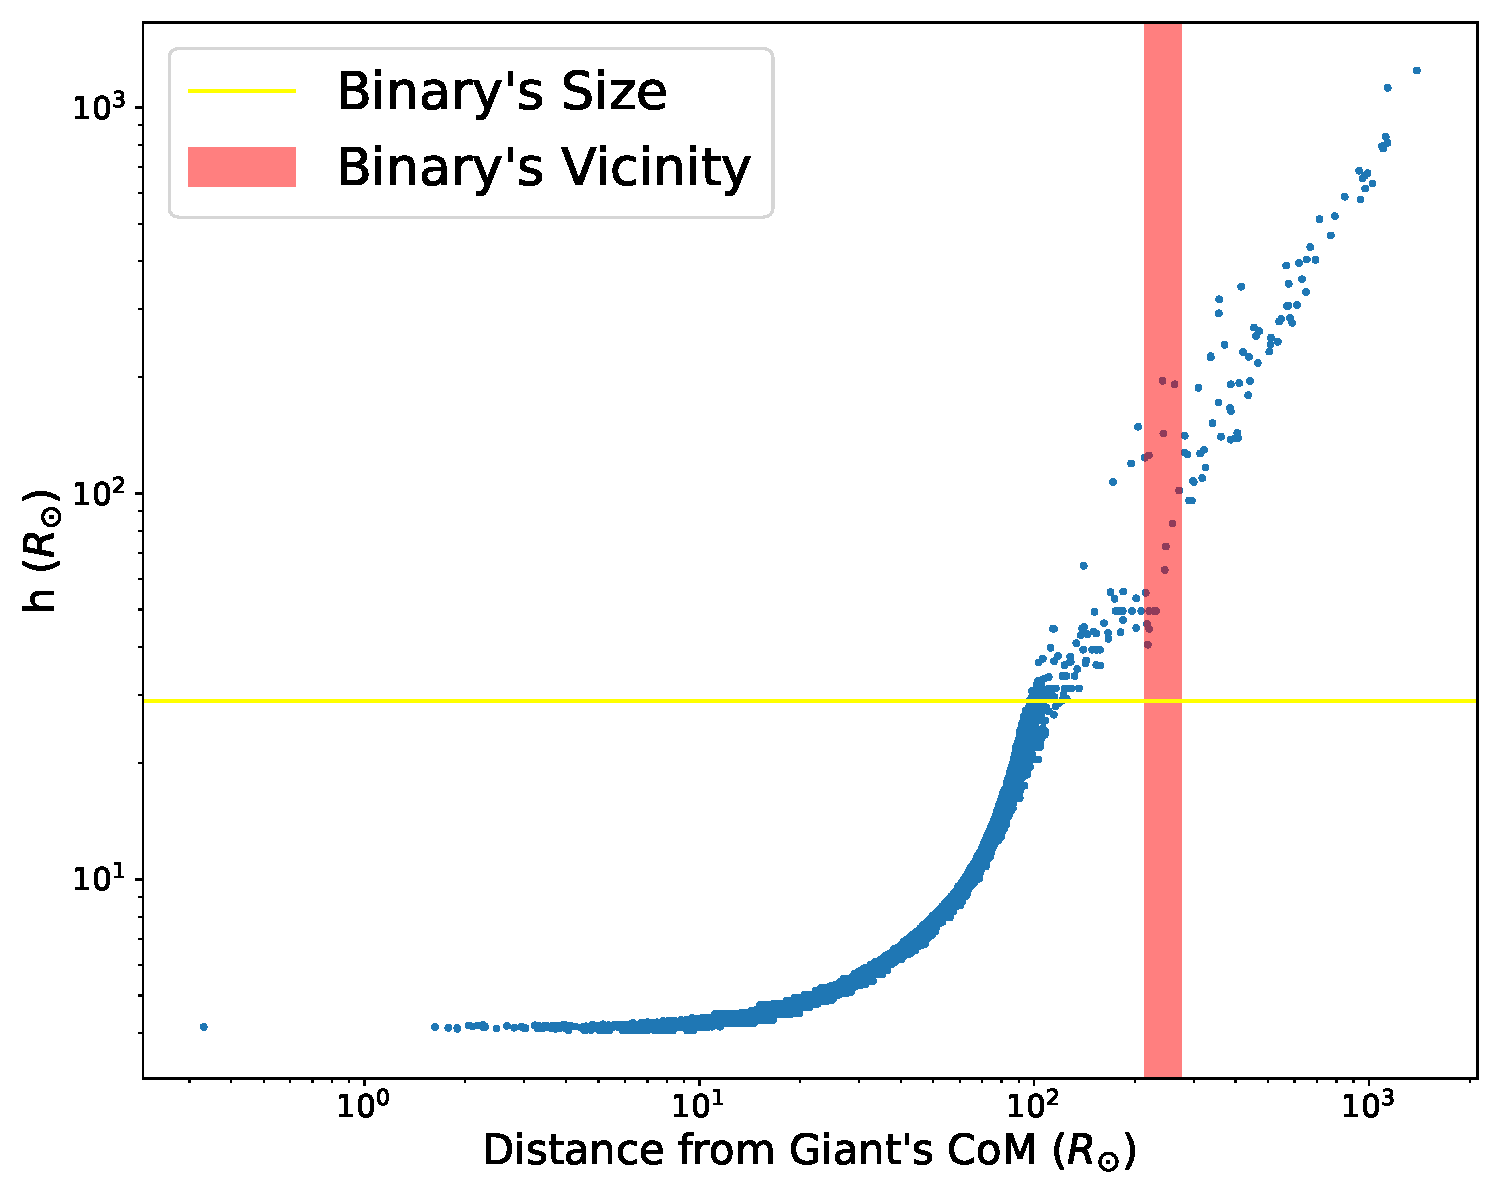
\includegraphics[width=0.9\textwidth]{Thesis/graphs/resolution_benchmark.pdf}
    \caption{Particles smoothing length in comparison to the binary's size at $t \approx 7.5$ yr, where the mass transfer is maximum.}
    \label{fig:resolution}
\end{figure}
Particles with smoothing lengths smaller than the binary's size, blue points bellow the yellow line, and close to the binary, blue point close/inside the red region, can influence hydrodynamically the inner orbit. At the current resolution, even when the mass transfer is maximum, the number of particles interacting with the binary is small (low-density mass stream), and thus their smoothing length is much larger than the size of the inner orbit. In conclusion, higher resolution simulations are required to safely estimate the evolution of the semi-major axis of the inner orbit.

When a gas particle is being accreted in the simulations, its mass and momentum are added to the star. However, because momentum is a vector, the star's acceleration or deceleration must be determined by the relative vector of the star's and the particle's velocity. Given the underestimating of gas drag and the resulting development illustrated in \cref{fig:accretion_inc_00_inner_semimajor_axis}, I ran a test simulation in which the angular momentum of the inner and outer orbits are antiparallel. The inner orbit contracts, as expected. In the case of parallel angular momentum vectors, accretion and gravitational interactions between the stars and the incoming mass stream appears to work as a slingshot effect in favor of the stars. Whereas in the antiparalel scenario, it appears to act as a braking mechanism for the stars.
\begin{figure}[!htb]
    \centering
    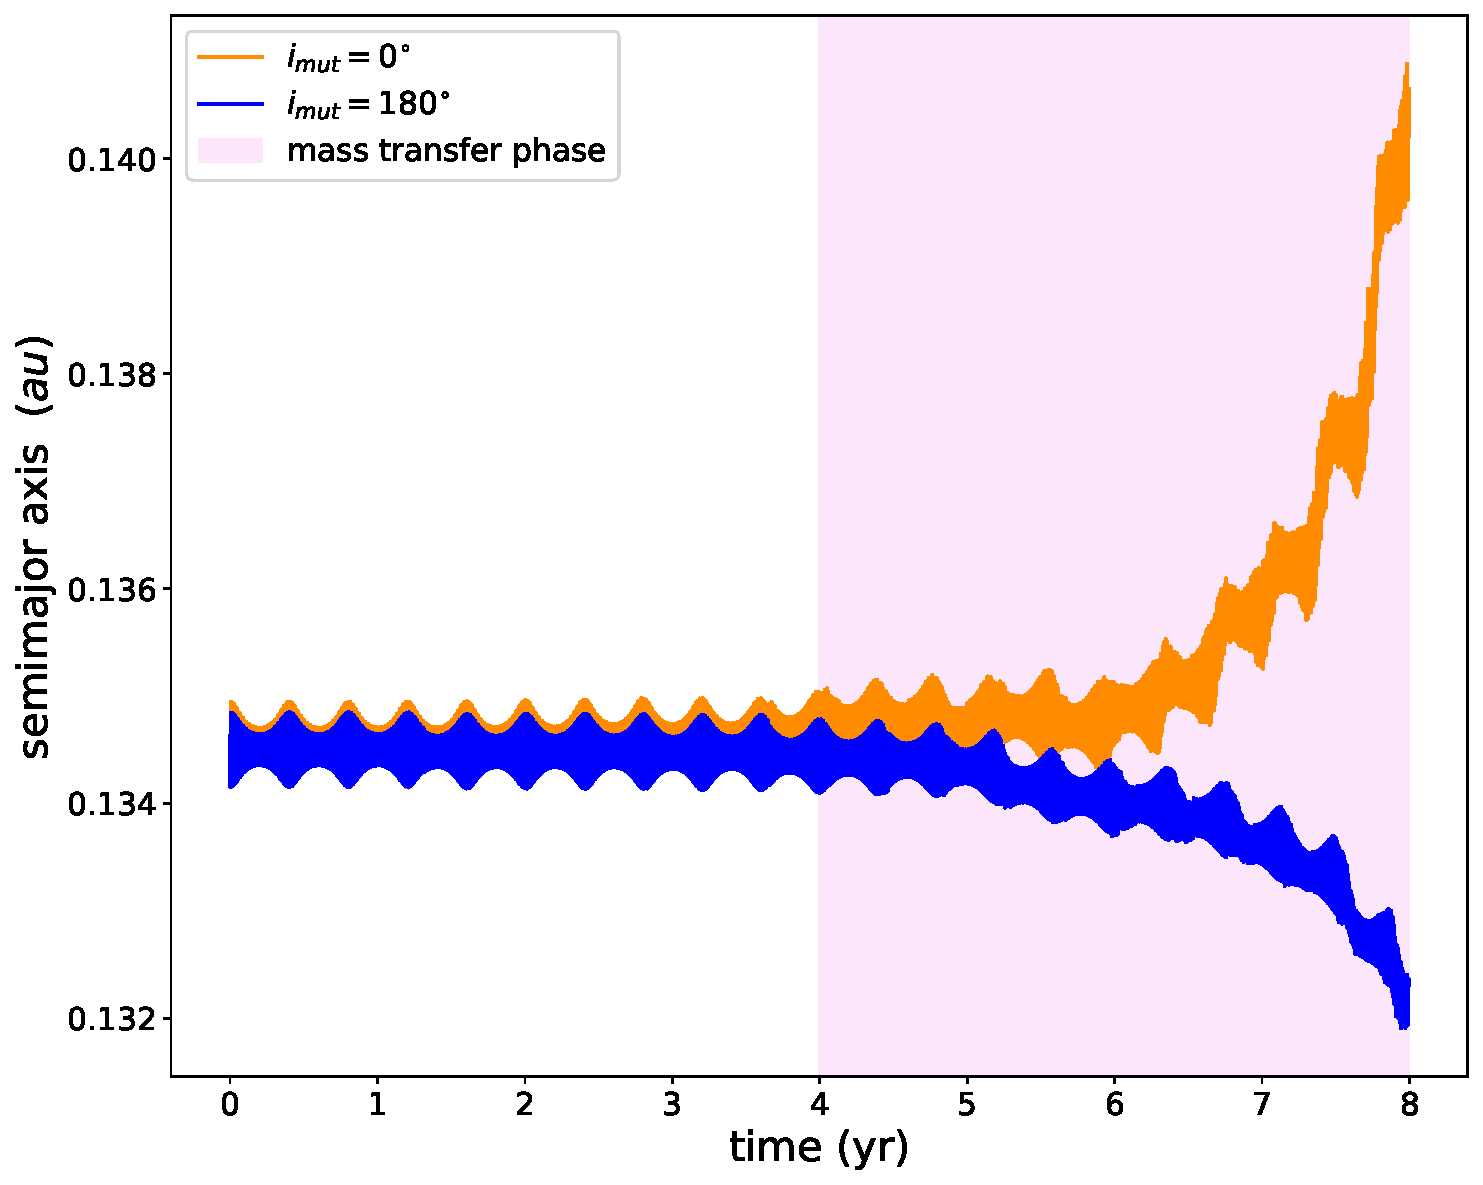
\includegraphics[width=0.9\textwidth]{Thesis/graphs/accretion_inc_00_retro_inner_semimajor_axis.pdf}
    \caption{Evolution of the semi-major axis of the inner orbit. The orbital angular momentum of the inner and outer orbit are parallel and antiparallel for the the orange and blue lines, respectively.}
    \label{fig:retro}
\end{figure}

Despite the fact that $N=50000$ is sufficient to initially resolve the giant at the moment of RLOF, see \cref{sec:1D_to_3D}, it is insufficient to accurately capture the gas drag on to the inner orbit. The fact that \cite{de2014evolution} use also $N=50000$ to examine mass transfer via RLOF by the outer star on the same system, was a motivation behind this particular choice. In their study, they employ a different SPH code. Nevertheless, both codes define the particles smoothing length in a similar fashion, thus it is a surprise that they are able to account for gas drag at seemingly the same resolution. 

To achieve higher resolution, I could simply increase the number of particles in my simulation. This is pretty straight forward in my code, however time restrictions require me to consider leaving this for future work. More specifically, with the available computational resources I obtain eight years of simulation in approximately five weeks of computational run time. Considering that the CPU time scales with the number of SPH particles as $NlogN$, increasing the number of particles by a factor of 5 results in several months of computational run time. 

In conclusion, with the current number of SPH particles the resolution of my simulations is probably insufficient to accurately capture the influence of the gas drag on the inner orbit. As a result, the gas drag is underestimated, while the models capture the gravitational interactions between the inner binary, the core of the tertiary, and its gaseous envelope. Regardless, I can still extract useful information about the evolution of the outer orbit and conjecture about the evolution of the inner orbit. 